\chapter{Introdução}

% [O problema]

O problema de evasão de discentes consiste no abandono, pelo discente, de um processo de estudos antes de sua conclusão. Essa definição pode ser detalhada especificando o escopo do processo de estudos: a evasão pode ser de um curso, de uma instituição de ensino, de cursos de uma determinada área, do sistema de ensino etc. O abandono do discente sem a conclusão do processo de estudos, considerando a finalidade desse processo, representa desperdício de recursos e de tempo de todos os envolvidos: discente, docentes, instituição de ensino e sociedade.

\todo{falar sobre estudos da pedagogia}

% [Justificativa]
O Programa de Apoio a Planos de Reestruturação e Expansão das Universidades Federais(REUNI), instituído pelo DECRETO Nº 6.096, DE 24 DE ABRIL DE 2007 \todo{como cita isso?}, possui como uma de suas diretrizes:

\begin{quote}
I - redução das taxas de evasão, ocupação de vagas ociosas e aumento de vagas de ingresso, especialmente no período noturno;
\end{quote}

\todo{sobre definições de evasão}

Na Universidade Federal do Ceará(UFC), de acordo com o Anuário estatístico \todo{quando sai o próximo?}de 2014, ano base 2013\todo{referenciar}, o indicador "Taxa de sucesso na graduação", definido como a proporção entre número de discentes diplomados e número de discentes ingressantes da graduação\todo{manual de indicadores do TCU, p.5}, esteve em 2013 com o menor valor desde 2008(Figura \ref{img:taxa-de-sucesso-ufc}). Já o indicador "Taxa de sucesso da graduação por curso", em 2013\todo{qual a definição?}, possuiu valor mínimo igual a 6.8\%, referente ao curso Ciências Sociais, habilitação em licenciatura(Tabela \ref{table:ts_2013}).

\begin{figure}[H]
	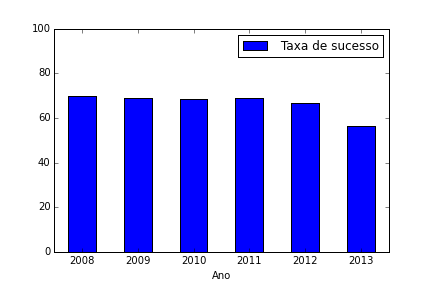
\includegraphics[scale=0.8]{img/taxa-de-sucesso-ufc.png}
	\caption{Taxa de Sucesso na Graduação - UFC}
	\label{img:taxa-de-sucesso-ufc}
\end{figure}

\begin{table}[H]
\begin{tabular}{llc}
\toprule
                            Curso &  Período & Taxa de Sucesso \\
\midrule
  Ciências Sociais - Licenciatura &  Noturno &            6.8\% \\
  Redes de Computadores - Quixadá &  Noturno &           13.3\% \\
          Geografia - Bacharelado &   Diurno &           15.3\% \\
        Letras - Português-Alemão &   Diurno &           17.6\% \\
           Engenharia Metalúrgica &   Diurno &           18.3\% \\
     Ciências Econômicas - Sobral &  Noturno &           20.9\% \\
 Sistemas de Informação - Quixadá &   Diurno &           22.0\% \\
          Filosofia - Bacharelado &  Noturno &           24.3\% \\
         Matemática - Bacharelado &   Diurno &           24.4\% \\
     Engenharia Elétrica - Sobral &   Diurno &           25.0\% \\
\bottomrule
\end{tabular}
\caption{Taxa de sucesso da graduação por curso na UFC em 2013 - 10 piores resultados, em ordem crescente}
\label{table:ts_2013}
\end{table}

Em DIRETRIZES GERAIS DO PROGRAMA DE APOIO A PLANOS DE REESTRUTURAÇÃO E EXPANSÃO DAS UNIVERSIDADES FEDERAIS REUNI p.4 \todo{referenciar}é ressaltado que o indicador "Taxa de conclusão dos cursos de graduação", cuja definição é igual à do "Taxa de Sucesso na graduação":

\begin{quote}
(...) não expressa diretamente as taxas de sucesso observadas nos cursos da universidade, ainda que haja uma relação estreita com fenômenos de retenção e evasão.
\end{quote}

Esse indicador não é sensível, por exemplo, à ocorrência de uma greve, fenômeno que causa atraso na formação dos discentes, podendo diminuir relevantemente a quantidade de diplomados em determinado ano. Funciona bem considerando o modelo em que, necessariamente, após a diplomação de uma turma de discentes, turma de igual tamanho irá ingressar. A realidade mostra que o processo de diplomação, iniciado com o ingresso do discente e finalizado com a emissão e recebimento de seu diploma, é mais complexo. Se adicionarmos o indivíduo que assume o papel de discente, a análise das causas da evasão torna-se mais complexa, trazendo à tona dimensões como a social e a econômica, além da vida pré universidade do indivíduo. Em \cite{unioeste}, por exemplo, informações sobre o trabalho do discente e se ele é casado foram os fatores mais relevantes na classificação dos discentes analisados com relação à evasão do curso. 

Uma das estratégias adotadas para diminuir as taxas de evasão é a identificação precoce de discentes com grande tendência para abandonarem seus cursos e a execução de ações que minimizem tal tendência. A identificação pode ser conduzida por observação do comportamento e resultados dos discentes, de forma subjetiva, pelos docentes e coordenadores de cursos, por exemplo. Em estudo realizado no departamento de engenharia elétrica da Eindhoven University of Technology\cite{Predicting_Students}, é relatado que em dezembro os discentes desse departamente recebem um aviso informando se são ou não aconselhados a continuarem no curso. Esse aviso é baseado na performance do discente no curso e em informações obtidas de professores do primeiro semestre e de discentes monitores. É relatado que o aviso parece ter bastante acurácia: geralmente discentes aconselhados a continuarem têm sucesso no próximo ano do curso, enquanto aqueles desaconselhados geralmente não continuam no curso.
Dois problemas decorrem dessa forma de identificação: sendo conduzida por pessoas, essa forma de identificação é limitada pelo conjunto de observações as quais o observador tem acesso; sendo subjetiva, seus resultados podem sofrer resistência para serem aceitos. A utilização de técnicas de aprendizado de máquina como forma de identificação pode contornar esses problemas, por, primeiro, fazer uso de dados registrados por sistemas de informação, provavelmente contendo informações mais amplas que as que uma pessoa pode observar; segundo, por fazer maior uso de dados registrados, sendo aceita mais facilmente como identificação objetiva. Nesse estudo foram utilizados diversos algoritmos de aprendizado de máquina com o objetivo de tentar detectar que um estudante irá abandonar seu curso. Foram utilizadas informações de discente referentes tanto ao período anterior ao seu ingresso na universidade, quanto ao posterior.

% [Objetivo]

Na UFC o estudo \cite{andriola} foi desenvolvido e objetivou analisar o problema da evasão de discentes através da análise da opinião de docentes e coordenadores sobre esse problema. O presente trabalho objetiva avaliar a aplicabilidade de técnicas de aprendizado de máquina ao problema de evasão de discentes na UFC a partir dos dados que seus sistemas de informação gerenciam. A UFC possui uma base de dados de informações sobre seus discentes gerada e mantida pelo sistema SIGAA(Sistema Integrado de Gestão de Atividades Acadêmicas). Para tanto é necessário que seja feito uma análise sobre a estrutura e qualidade dos dados disponíveis.

% [Definição de termos]

% [Importância]